\documentclass{article}    
\usepackage[letterpaper,margin=1in]{geometry}
\usepackage{lastpage}
\usepackage{graphicx}
\usepackage{fancyhdr}
\usepackage{enumitem}
\usepackage{amssymb}
\usepackage{amsmath}

\def\ojoin{\setbox0=\hbox{$\bowtie$}%
  \rule[-.02ex]{.25em}{.4pt}\llap{\rule[\ht0]{.25em}{.4pt}}}
\def\leftouterjoin{\mathbin{\ojoin\mkern-5.8mu\bowtie}}
\def\rightouterjoin{\mathbin{\bowtie\mkern-5.8mu\ojoin}}
\def\fullouterjoin{\mathbin{\ojoin\mkern-5.8mu\bowtie\mkern-5.8mu\ojoin}}

\fancypagestyle{plain}{%
\fancyhf{}%
\lhead{ECS165A SQ18}
\rhead{\today}
\cfoot{Homework 4\\ \thepage\ of \pageref{LastPage} }
\renewcommand{\headrulewidth}{0.4pt}
\renewcommand{\footrulewidth}{0.4pt}
}

\pagestyle{fancy}
\fancyhf{}
\lhead{ECS165A SQ18}
\rhead{\today}
\cfoot{Homework 4\\ \thepage\ of \pageref{LastPage} }
\renewcommand{\headrulewidth}{0.4pt}
\renewcommand{\footrulewidth}{0.4pt}

\begin{document}

\title{Homework 4}
\author{Name: Mengfei Lan HERE\\SID: 916726216\\Partner Name: Yu Deng\\Partner SID: 913208229}

\maketitle

Due 11:59PM June 5, 2018. {\bf READ ALL DIRECTIONS VERY CAREFULLY!} 
Submit your code, tex files along with a generated PDF. {\bf DO NOT SUBMIT DATA FILES!} 
For this homework you will be working in groups of two, a group of three will only be allowed with approval due to odd number of students. 
All programs will be evaluated on the CSIF. Upload your files as a tar gzip file (tgz). Only submit one homework per partner. This specification is subject to change.

You are designing a database for a university called FakeU. As a trial you have been provided grade data from courses for departments ABC and DEF. 
The grade data is from Summer of 1989 until Summer of 2012. The data provided is in CSV format, and is only as complete as could be made possible. 
There may be errors, omissions or redundant data in the files. 
FakeU like UC Davis is on a quarter system, however they have recently transitioned to a single summer quarter instead of two summer sessions. 
This has corrupted some of their summer data as all summer session classes have now been grouped into a single summer quarter term. 
Each course has a course ID (CID), a term it was offered (TERM), a subject (SUBJ), a course number (CRSE), a section (SEC), and number of units (UNITS). 
Within a course there listings of meetings, the instructor of the meeting (INSTRUCTOR(S)), meeting type (TYPE), day of meeting (DAYS), time of meeting (TIME), meeting building (BUILD), and meeting room (ROOM) are also listed. For each student that takes the course there is a student seat (SEAT), a student ID (SID), the student�s surname (SURNAME), the student�s preferred name (PREFNAME), the student�s (LEVEL), the number of units the student is receiving (UNITS), the student�s class standing (CLASS), the student�s major (MAJOR), the grade the student received in the course (GRADE), the student�s registration status (STATUS), and the student�s e-mail address (EMAIL).
There may be courses that are cross listed between the two departments (e.g. ABC 123 may be cross listed as DEF 456).

You {\bf MUST} put each problem on a separate page with 1a on the second page, for example 1a will be on page 2 and 1b will be on page 3 (this template is already setup for this). 
You {\bf MUST} put your name and student ID in the provided author section above. {\bf FAILURE TO DO SO MAY RESULT IN NO CREDIT!} 
The data will be provided on Canvas, and the CSV files will also be on the CSIF in /home/cjnitta/ecs165a/Grades. All submissions will be compared with MOSS, including against past submissions.

Some useful tips: 
\begin{itemize}
\item When loading the tuples into the database, insert them in batches. Inserting one tuple at a time may cause the program to take on the order of tens of minutes or hours instead of a few minutes.
\item Test a subset of the data first.
\end{itemize}

\clearpage
\section*{Part 1}
You will be creating a database schema for your grade data.

\begin{enumerate}[label=\alph*.]
\item Provide an ER diagram for your database schema. Only include images generated from vector based programs. \\
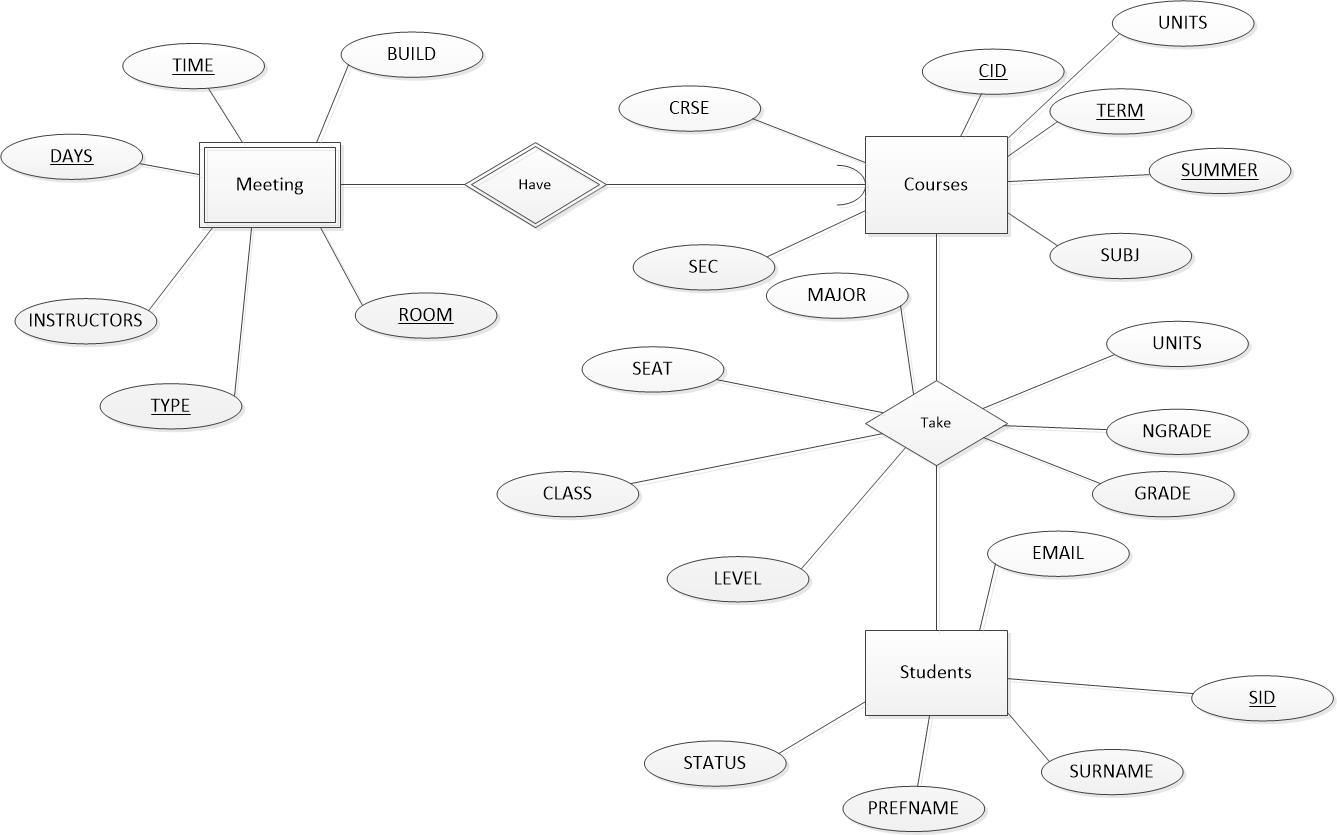
\includegraphics[width=6in,height=4in]{ER diagram.jpg} \clearpage
\item Provide a description of the tables in your schema, and their attributes. Make sure you describe how you will store the instructor, student, building, course, etc. information. \\
Courses(\underline{CID}, \underline{TERM}, SUBJ, CRSE, SEC, UNITS, \underline{SUMMER})\\
Students(\underline{SID}, SURNAME, PREFNAME, STATUS, EMAIL)\\
Take(\underline{CID}, \underline{SID}, \underline{TERM}, MAJOR, UNITS, GRADE, SEAT, CLASS, LEVEL, NGRADE, \underline{SUMMER})\\
Meeting(INSTRUCTORS, \underline{TYPE}, \underline{DAYS}, \underline{TIME}, BUILD, ROOM, \underline{CID},\underline{SUMMER},\underline{TERM})\\

Convert the ER diagram to four relations as above.\\\\ 
We plan to create four tables in the database. The first one named Courses, includes six attributes--CID, TERM, SUBJ, CRSE, SEC, UNITS, and its key is {CID,TERM,SUMMER}. The second one named Students, includes eight attributes--SID, SURNAME, PREFNAME, LEVEL, CLASS, MAJOR, STATUS, EMAIL, and its key is SID. The third one named Take, and it stores information about which courses are chosen by which student. This table is got for many-many weak relationship Take, and it includes four attributes--CID, SID, UNITS, GRADE, SEAT. Its key is {CID, SID, TERM,SUMMER}. The last one named Meeting, which is a weak entity. It includes nine attributes--INSTRUCTORS, TYPE, DAYS, TIME, BUILD, ROOM, CID, SUMMER, TERM, and its key is {TYPE, DAYS, TIME, CID, SUMMER, TERM}.     \clearpage
\item What are the functional (and multivalue) dependencies that you expect to hold for each relation if any. If you don't expect any to hold, describe why not. \\
Functional dependencies we want to hold:\\
1. TERM, SUMMER, CID $\rightarrow$ UNITS, SUBJ, SEC, CRSE\\
2. CID, TERM, SUMMER, SID $\rightarrow$ MAJOR, SEAT, CLASS, UNITS, NGRADE, GRADE\\
3. SID $\rightarrow$ EMAIL, STATUS, PREFNAME, SURNAME\\
4. TERM, SUMMER, ROOM, CID, TIME, DAYS, TYPE $\rightarrow$ BUILD, INSTRUCTORS\\ \clearpage
\end{enumerate}

\section*{Part 2} 
Write a program to load the grade data into a PostgreSQL database called FakeUData that follows your schema.
You {\bf MUST} use the database called FakeUData, and should assume it will already be created for you without any tables or data in it.
You may {\bf NOT} hardcode usernames in your code, use the USER environmental variable instead if user is needed.
Your program can be written in C++ or python, you may {\bf NOT} use standalone SQL or text files that hold your queries. 
You may {\bf NOT} use shell calls to implement your program.
All your queries need to be in your code. 
If you choose to make a C++ program, you must include a makefile and call the program loadfakeu. 
Include a readme file with descriptions of any issues/problems. 
If you choose to make a python program you must specify which version of python you used, and must provide a loadfakeu bash script to launch your python program.
The loadfakeu program {\bf MUST} be able to take one optional argument (the directory where the CSV data files will be located). 
If the argument is omitted, the default is the current working directory.
Scripts that require greater than 10 minutes to load all of the data may lose points. 
\clearpage

\section*{Part 3}
Write another program to query your database to calculate the following values, put the results in your write up, some may be best described with a chart instead of raw values. 
Name your program queryfakeu, it must output the data values for the following queries. 
The query program does not have to do everything in the SQL queries, but should limit the amount of data transfered. 
For example it is acceptable to have one SQL query for each unit number (1 - 20) for 3a, but it would be unacceptable to pull all student data on a per student basis and calculate the results. 
\begin{enumerate}[label=\alph*.]
\item Calculate the percent of students that attempt 1 � 20 units of ABC or DEF per quarter for every unit increment (e.g. 1, 2, 3,�). \\
unit is: 1.0, percentage is: 1.57\% \\
unit is: 2.0, percentage is: 0.41\% \\
unit is: 3.0, percentage is: 1.66\% \\
unit is: 4.0, percentage is: 45.2\% \\
unit is: 5.0, percentage is: 3.03\% \\
unit is: 6.0, percentage is: 1.28\% \\
unit is: 7.0, percentage is: 1.97\% \\
unit is: 8.0, percentage is: 12.6\% \\
unit is: 9.0, percentage is: 3.64\% \\
unit is: 10.0, percentage is: 1.55\% \\
unit is: 11.0, percentage is: 1.99\% \\
unit is: 12.0, percentage is: 13.9\% \\
unit is: 13.0, percentage is: 5.58\% \\
unit is: 14.0, percentage is: 1.82\% \\
unit is: 15.0, percentage is: 0.98\% \\
unit is: 16.0, percentage is: 1.36\% \\
unit is: 17.0, percentage is: 0.73\% \\
unit is: 18.0, percentage is: 0.15\% \\
unit is: 19.0, percentage is: 0.08\% \\
unit is: 20.0, percentage is: 0.05\% \\
 \clearpage
\item Find the easiest and hardest instructors based upon the grades of all the students they have taught in their courses. Provide their name and the average grade they assigned. (Ignore P/NP, S/NS grades) \\
Easiest:\\
professor is: Odonnell, Madison G. and the gpa is: 3.95\\
professor is: Russo, Angel J. and the gpa is: 3.95\\
\\\\
Hardest:\\
professor is: Turner, Emily A. and the gpa is: 1.7\\

 \clearpage
\item Calculate the average GPA for the students that take each number of units from part a. Assume that the grades have standard grade points (A+ = 4.0, A = 4.0, A- = 3.7, B+ = 3.3�). \\
unit is: 1.0, average gpa is: 3.74\\
unit is: 2.0, average gpa is: 3.739\\
unit is: 3.0, average gpa is: 3.606\\
unit is: 4.0, average gpa is: 2.767\\
unit is: 5.0, average gpa is: 2.659\\
unit is: 6.0, average gpa is: 3.534\\
unit is: 7.0, average gpa is: 3.164\\
unit is: 8.0, average gpa is: 2.362\\
unit is: 9.0, average gpa is: 2.936\\
unit is: 10.0, average gpa is: 3.013\\
unit is: 11.0, average gpa is: 2.967\\
unit is: 12.0, average gpa is: 2.363\\
unit is: 13.0, average gpa is: 2.708\\
unit is: 14.0, average gpa is: 2.872\\
unit is: 15.0, average gpa is: 2.977\\
unit is: 16.0, average gpa is: 2.480\\
unit is: 17.0, average gpa is: 2.886\\
unit is: 18.0, average gpa is: 2.992\\
unit is: 19.0, average gpa is: 3.061\\
unit is: 20.0, average gpa is: 2.583\\

 \clearpage
\item Find the courses with the highest and lowest pass rates. Assume that F, NP, and NS are not passing grades. \\
result for 3d(highest):\\
 ABC110 100.0\%, 
 ABC111 100.0\%, 
 ABC112 100.0\%, 
 ABC113 100.0\%, 
 ABC114 100.0\%, 
 ABC215 100.0\%, 
 ABC223 100.0\%, 
 ABC225 100.0\%, 
 ABC231 100.0\%, 
 ABC233 100.0\%, 
 ABC244 100.0\%, 
 ABC249 100.0\%, 
 ABC250 100.0\%, 
 ABC252 100.0\%, 
 ABC255 100.0\%, 
 ABC256 100.0\%, 
 ABC258 100.0\%, 
 ABC259 100.0\%, 
 ABC260 100.0\%, 
 ABC302 100.0\%, 
 ABC303 100.0\%, 
 ABC311 100.0\%, 
 ABC313 100.0\%, 
 ABC315 100.0\%, 
 ABC317 100.0\%, 
 ABC318 100.0\%, 
 ABC321 100.0\%, 
 ABC323 100.0\%, 
 ABC326 100.0\%, 
 ABC327 100.0\%, 
 ABC328 100.0\%, 
 ABC333 100.0\%, 
 ABC334 100.0\%, 
 ABC340 100.0\%, 
 ABC341 100.0\%, 
 ABC342 100.0\%, 
 ABC343 100.0\%, 
 ABC345 100.0\%, 
 ABC346 100.0\%, 
 ABC349 100.0\%, 
 ABC351 100.0\%, 
 ABC352 100.0\%, 
 ABC353 100.0\%, 
 ABC357 100.0\%, 
 ABC358 100.0\%, 
 ABC359 100.0\%, 
 ABC361 100.0\%, 
 ABC362 100.0\%, 
 ABC364 100.0\%, 
 ABC368 100.0\%, 
 ABC369 100.0\%, 
 ABC372 100.0\%, 
 ABC373 100.0\%, 
 ABC374 100.0\%, 
 ABC377 100.0\%, 
 DEF105 100.0\%, 
 DEF202 100.0\%, 
 DEF213 100.0\%, 
 DEF216 100.0\%, 
 DEF217 100.0\%, 
 DEF218 100.0\%, 
 DEF224 100.0\%, 
 DEF236 100.0\%, 
 DEF237 100.0\%, 
 DEF240 100.0\%, 
 DEF255 100.0\%, 
 DEF260 100.0\%, 
 DEF272 100.0\%, 
 DEF278 100.0\%, 
 DEF282 100.0\%, 
 DEF288 100.0\%, 
 DEF292 100.0\%, 
 DEF293 100.0\%, 
 DEF295 100.0\%, 
 DEF298 100.0\%, 
 DEF302 100.0\%, 
 DEF303 100.0\%, 
 DEF304 100.0\%, 
 DEF305 100.0\%, 
 DEF306 100.0\%, 
 DEF307 100.0\%, 
 DEF310 100.0\%, 
 DEF313 100.0\%, 
 DEF314 100.0\%, 
 DEF316 100.0\%, 
 DEF319 100.0\%, 
 DEF320 100.0\%, 
 DEF322 100.0\%, 
 DEF323 100.0\%, 
 DEF324 100.0\%, 
 DEF325 100.0\%, 
 DEF328 100.0\%, 
 DEF329 100.0\%, 
 DEF330 100.0\%, 
 DEF332 100.0\%, 
 DEF333 100.0\%, 
 DEF337 100.0\%, 
 DEF338 100.0\%, 
 DEF339 100.0\%, 
 DEF341 100.0\%, 
 DEF343 100.0\%, 
 DEF345 100.0\%, 
 DEF348 100.0\%, 
 DEF349 100.0\%, 
 DEF351 100.0\%, 
 DEF352 100.0\%, 
 DEF353 100.0\%, 
 DEF354 100.0\%, 
 DEF355 100.0\%, 
 DEF362 100.0\%, 
 DEF363 100.0\%, 
 DEF364 100.0\%, 
 DEF365 100.0\%, 
 DEF366 100.0\%, 
 DEF368 100.0\%, 
 DEF369 100.0\%, 
 DEF375 100.0\%, 
 DEF376 100.0\%, 
 DEF378 100.0\%, 
 DEF380 100.0\%, 
 DEF381 100.0\%, 
 DEF382 100.0\%, 
 DEF386 100.0\%, 
 DEF387 100.0\%, 
 DEF388 100.0\%, 
 DEF390 100.0\%, 
 DEF393 100.0\%, 
 DEF397 100.0\%, 
 DEF398 100.0\%, 
 DEF401 100.0\%, 
 DEF403 100.0\%, 
 DEF404 100.0\%, 
 DEF408 100.0\%, 
 DEF410 100.0\%, 
 DEF411 100.0\%, 
 DEF412 100.0\%, 
 DEF414 100.0\%, 
 DEF415 100.0\%, 
 DEF419 100.0\%, 
 DEF420 100.0\%, 
 DEF422 100.0\%, 
 DEF423 100.0\%, 
 DEF424 100.0\%, 
 DEF425 100.0\%, \\
result for 3d(lowest):\\
 DEF108 50.0\%, 
 \clearpage
\item Find the list of courses that must be cross listed as they have the same meeting times during the normal quarters. Only list the pair once, put the course name/number string in alphabetically order of the pairs. \\
ABC216 is cross listed with DEF254 \\
ABC218 is cross listed with DEF255 \\
ABC337 is cross listed with DEF381 \\
 \clearpage
\item Find the major that performs the best/worst on average in ABC courses. Repeat the analysis for DEF courses as well. \\
perform the best on average in ABC courses: \\
major is: O207 and its average gpa is: 4.0\\
major is: O176 and its average gpa is: 4.0\\
major is: O100 and its average gpa is: 4.0\\
major is: O179 and its average gpa is: 4.0\\
major is: O139 and its average gpa is: 4.0\\
major is: O255 and its average gpa is: 4.0\\
major is: O171 and its average gpa is: 4.0\\
major is: O169 and its average gpa is: 4.0\\
major is: O113 and its average gpa is: 4.0\\
major is: O167 and its average gpa is: 4.0\\
major is: O275 and its average gpa is: 4.0\\
major is: O151 and its average gpa is: 4.0\\
major is: O193 and its average gpa is: 4.0\\
==============================\\
\\
perform the worst on average in ABC courses: \\
major is: O279 and its average gpa is: 0.0\\
major is: O152 and its average gpa is: 0.0\\
major is: O263 and its average gpa is: 0.0\\
major is: O281 and its average gpa is: 0.0\\
==============================\\
\\
perform the best on average in DEF courses: \\
major is: O278 and its average gpa is: 4.0\\
major is: O135 and its average gpa is: 4.0\\
major is: O195 and its average gpa is: 4.0\\
major is: OT63 and its average gpa is: 4.0\\
major is: O264 and its average gpa is: 4.0\\
major is: OT87 and its average gpa is: 4.0\\
major is: O122 and its average gpa is: 4.0\\
major is: OT51 and its average gpa is: 4.0\\
==============================\\
result for 3f\\
perform the worst on average in DEF courses: \\
major is: OT95 and its average gpa is: 0.0\\
major is: OT45 and its average gpa is: 0.0\\
major is: O106 and its average gpa is: 0.0\\
 \clearpage
\item Find the top 5 majors that students transfer from into ABC. What is the percent of students from each of those majors compared to overall transfers? \\
major is: OT16 and percentage is: 14.0\% \\
major is: DEF2 and percentage is: 10.4\% \\
major is: OT26 and percentage is: 7.69\% \\
major is: OT35 and percentage is: 7.19\% \\
major is: DEF1 and percentage is: 3.10\% \\
 \clearpage
\item Find the top 5 majors that students transfer to from ABC. What is the percent of students to each of those majors compared to overall transfers out? \\
major is: DEF1 and percentage is: 5.11\% \\
major is: DEF2 and percentage is: 4.18\% \\
major is: OTH8 and percentage is: 3.82\% \\
major is: O174 and percentage is: 2.43\% \\
major is: OT35 and percentage is: 1.58\% \\
 \clearpage
\end{enumerate}

\section*{Part 4}
Extra credit: The Efficient XML Interchange (EXI) is a format for the compact representation of XML information. 
The CSV files provided for this assignment have been consolidated into a single EXI file (HW4Grades.exi) that is available in the resources section of Canvas. 
Implement a separate program that it can load the database from the EXI file. 
You may {\bf NOT} use shell calls, or creation of external temporary files for this part.
Name your program or bash script loadfakeuexi.
\clearpage

\section*{Part 5}
Extra credit: Additional queries/query program.
\begin{enumerate}[label=\alph*.]
\item Find the courses that appear to be prerequisites for ABC 203, ABC 210, and ABC 222. For this problem list the courses that the X\% of students have taken for every 5\% increment from 50\% - 100\% prior to taking the course. (Add this output to your query program.)\\
50\% - 55\%:\\
52.77\% of the students have taken 107ABC before taking 210ABC\\
54.88\% of the students have taken 105ABC before taking 210ABC\\
53.30\% of the students have taken 202ABC before taking 222ABC\\
\\
\\
55\% - 60\%:\\
55.93\% of the students have taken 202ABC before taking 210ABC\\
57.85\% of the students have taken 107ABC before taking 222ABC\\
\\
\\
60\% - 65\%:\\
63.16\% of the students have taken 209ABC before taking 222ABC\\
63.09\% of the students have taken 105ABC before taking 222ABC\\
\\
\\
65\% - 70\%:\\
\\
\\
70\% - 75\%:\\
70.44\% of the students have taken 106ABC before taking 210ABC\\
\\
\\
75\% - 80\%:\\
77.83\% of the students have taken 221ABC before taking 210ABC\\
78.62\% of the students have taken 104ABC before taking 210ABC\\
\\
\\
80\% - 5\%:\\
80.74\% of the students have taken 106ABC before taking 222ABC\\
\\
\\
85\% - 90\%:\\
86.34\% of the students have taken 104ABC before taking 222ABC\\
\\
\\
90\% - 95\%:\\
92.08\% of the students have taken 108ABC before taking 210ABC\\
\\
\\
95\% - 100\%:\\
96.56\% of the students have taken 209ABC before taking 210ABC\\
99.11\% of the students have taken 221ABC before taking 222ABC\\
97.31\% of the students have taken 108ABC before taking 222ABC\\
 \clearpage
\item Write a program that will find an open room for course expansion. The program must prompt for term, CID, and number students to add. The room(s) returned should be ordered from best to worst fit with up to 5 results. Assume that each room capacity is the maximum number of students listed for any particular meeting in the data files (don't forget that lectures may be split across multiple CIDs). Name this program findroomfakeu.
\footnotesize
for build LH5 room 23the capacity is: 10 people.\\
for build TB3 room 167the capacity is: 54 people.
for build LH5 room 26the capacity is: 180 people.\\
for build LH1 room 38the capacity is: 18 people.
for build MB3 room 1066the capacity is: 185 people.\\
for build MB5 room 1328the capacity is: 54 people.
for build LH4 room 51the capacity is: 108 people.\\
for build TB3 room 139the capacity is: 17 people.
for build LH5 room 3the capacity is: 378 people.\\
for build TB2 room 112the capacity is: 180 people.
for build LH5 room 31the capacity is: 18 people.\\
for build MB5 room 1352the capacity is: 38 people.
for build LH5 room 41the capacity is: 15 people.\\
for build LH1 room 94the capacity is: 270 people.
for build LH5 room 9the capacity is: 270 people.\\
for build MB2 room 1014the capacity is: 195 people.
for build LH5 room 18the capacity is: 54 people.\\
for build MB4 room 3008the capacity is: 108 people.
for build LH1 room 62the capacity is: 215 people.\\
for build LH5 room 17the capacity is: 14 people.
for build LH2 room 28the capacity is: 50 people.\\
for build LH4 room 41the capacity is: 12 people.
for build TB3 room 132the capacity is: 198 people.\\
for build MB4 room 2240the capacity is: 378 people.
for build LH1 room 66the capacity is: 54 people.\\
for build LH1 room 70the capacity is: 22 people.
for build TB4 room 103the capacity is: 108 people.\\
for build LH1 room 82the capacity is: 36 people.
for build MB4 room 2250the capacity is: 270 people.\\
for build LH1 room 34the capacity is: 54 people.
for build LH4 room 63the capacity is: 180 people.\\
for build LH4 room 67the capacity is: 180 people.
for build LH5 room 50the capacity is: 108 people.\\
for build MB5 room 1324the capacity is: 50 people.
for build MB4 room 1045the capacity is: 48 people.\\
for build LH4 room 71the capacity is: 108 people.
for build LH3 room 58the capacity is: 378 people.\\
for build TB3 room 118the capacity is: 180 people.
for build LH2 room 20the capacity is: 63 people.\\
for build LH2 room 22the capacity is: 46 people.
for build TB3 room 111the capacity is: 102 people.\\
for build LH4 room 37the capacity is: 17 people.
for build LH5 room 44the capacity is: 18 people.\\
for build MB6 room 1144the capacity is: 108 people.
for build LH4 room 45the capacity is: 270 people.\\
for build LH5 room 29the capacity is: 18 people.
for build LH3 room 56the capacity is: 34 people.\\
for build TB3 room 146the capacity is: 15 people.
for build LH5 room 14the capacity is: 378 people.\\
for build MB3 room 1082the capacity is: 371 people.
for build TB3 room 125the capacity is: 54 people.\\
for build MB3 room 1062the capacity is: 215 people.
for build TB4 room 108the capacity is: 270 people.\\
for build TB2 room 118the capacity is: 42 people.
for build  room the capacity is: 155376 people.\\
for build TB2 room 110the capacity is: 270 people.
for build LH5 room 33the capacity is: 108 people.\\
for build LH1 room 42the capacity is: 42 people.
for build MB1 room 1030the capacity is: 54 people.\\
for build LH5 room 19the capacity is: 108 people.
for build LH5 room 24the capacity is: 12 people.\\
for build MB2 room 1008the capacity is: 36 people.
for build LH5 room 6the capacity is: 180 people.\\
for build MB5 room 1320the capacity is: 30 people.
for build LH5 room 49the capacity is: 180 people.\\
for build LH5 room 45the capacity is: 18 people.
for build LH5 room 11the capacity is: 18 people.\\
for build LH4 room 39the capacity is: 34 people.
for build LH2 room 18the capacity is: 52 people.\\
for build LH5 room 34the capacity is: 180 people.
for build MB6 room 1139the capacity is: 192 people.\\
for build LH3 room 62the capacity is: 198 people.
for build LH5 room 28the capacity is: 48 people.\\
for build LH4 room 55the capacity is: 54 people.
for build LH5 room 47the capacity is: 108 people.\\
for build LH5 room 5the capacity is: 13 people.
for build LH5 room 32the capacity is: 50 people.\\
for build LH1 room 46the capacity is: 434 people.
for build TB2 room 116the capacity is: 52 people.\\
for build LH1 room 58the capacity is: 8 people.
for build LH1 room 86the capacity is: 34 people.\\
for build MB2 room 1002the capacity is: 225 people.
for build LH5 room 22the capacity is: 378 people.\\
for build LH5 room 20the capacity is: 17 people.
for build LH5 room 48the capacity is: 18 people.\\
for build TB3 room 160the capacity is: 15 people.
for build MB1 room 1040the capacity is: 108 people.\\
for build LH5 room 2the capacity is: 54 people.
for build MB4 room 2270the capacity is: 15 people.\\
for build LH2 room 26the capacity is: 14 people.
for build MB2 room 1016the capacity is: 240 people.\\
for build LH1 room 130the capacity is: 18 people.
for build LH5 room 25the capacity is: 12 people.\\
for build LH5 room 38the capacity is: 180 people.
for build LH4 room 43the capacity is: 270 people.\\
for build MB6 room 1149the capacity is: 180 people.
for build TB2 room 114the capacity is: 180 people.\\
for build LH1 room 90the capacity is: 38 people.
for build MB5 room 1356the capacity is: 108 people.\\
for build LH5 room 13the capacity is: 18 people.
for build MB4 room 2230the capacity is: 378 people.\\
for build MB4 room 2280the capacity is: 18 people.
for build LH5 room 7the capacity is: 18 people.\\
for build LH1 room 78the capacity is: 14 people.
for build MB2 room 1012the capacity is: 44 people.\\
for build MB2 room 1004the capacity is: 108 people.
for build LH5 room 15the capacity is: 18 people.\\
for build MB3 room 1070the capacity is: 378 people.
for build LH5 room 42the capacity is: 108 people.\\
for build LH1 room 54the capacity is: 11 people.
for build LH5 room 21the capacity is: 7 people.\\
for build LH1 room 14the capacity is: 270 people.
for build MB4 room 1060the capacity is: 245 people.\\
for build TB3 room 153the capacity is: 18 people.
for build LH1 room 138the capacity is: 3 people.\\
for build MB4 room 1055the capacity is: 240 people.
for build LH5 room 16the capacity is: 14 people.\\
for build LH1 room 74the capacity is: 18 people.
for build MB4 room 2300the capacity is: 13 people.\\
for build LH1 room 118the capacity is: 15 people.
for build TB1 room 105the capacity is: 180 people.\\
for build LH5 room 40the capacity is: 18 people.
for build MB2 room 1018the capacity is: 42 people.\\
for build MB5 room 1332the capacity is: 270 people.
for build LH1 room 110the capacity is: 54 people.\\
for build LH5 room 10the capacity is: 18 people.
for build TB3 room 174the capacity is: 108 people. \clearpage
\end{enumerate}



\end{document}